% !TeX root = ./../memoria.tex
\chapter{Introducción general}

\label{Capitulo1}

\newcommand{\keyword}[1]{\textbf{#1}}
\newcommand{\tabhead}[1]{\textbf{#1}}
\newcommand{\code}[1]{\texttt{#1}}
\newcommand{\file}[1]{\texttt{\bfseries#1}}
\newcommand{\option}[1]{\texttt{\itshape#1}}
\newcommand{\grados}{$^{\circ}$}

En este capítulo se introduce al campo de estudio de la robótica móvil. Se aborda una comparación entre diferentes plataformas didácticas comerciales y se exponen el alcance y las motivaciones que llevaron al desarrollo del presente proyecto.

\section{Robótica móvil}

La robótica móvil se encarga del estudio de los robots móviles y hace especial hincapié en el desarrollo de capacidades les permitan decidir de manera autónoma cómo, cuándo y a dónde moverse.

En contraste con los robots manipuladores cuya base se encuentra fija con respecto a un sistema de referencia, los robots móviles son aquellos capaces de moverse de un lugar a otro. Esta particularidad los obliga a ser capaces de interactuar con entornos no determinísticos, es decir, propensos a situaciones impredecibles como por ejemplo una puerta entreabierta, un objeto o persona que obstaculiza el camino, etc.

\subsection{Tipos de robots móviles}

Dependiendo de cómo realizan su locomoción, es posible caracterizar a los robots móviles en los siguientes tipos:
\begin{itemize}
	\item{Robots con patas}
	\item{Robots aéreos}
	\item{Robots con ruedas}
\end{itemize}

Cada uno de estos tipos plantea su propio conjunto de ventajas y desventajas, así como dificultades para su implementación. En el presente trabajo se hizo énfasis solo en el último tipo de la lista, es decir en los robots con ruedas.

\newpage

\section{Estado del arte}

Existe una amplia gama de robots móviles con ruedas ofrecidos específicamente para el sector académico. A continuación se presenta un breve sumario de opciones que se encuentran actualmente en el mercado.

\subsection{TurtleBot}\label{sec:turtlebot}

TurtleBot constituye una familia de robots móviles para uso personal de bajo costo. Su uso se extiende tanto a la academia como a roboticistas aficionados en todo el mundo.

Aunque su primera iteración vio la luz en 2010 con un conjunto de características bastante modestas, el lanzamiento de nuevas versiones le aseguró su lugar como dispositivo de referencia dentro de la plataforma ROS.

Muchas de las consideraciones de diseño del robot propuesto en este trabajo fueron tomados de este modelo por lo que se espera que se encuentren similitudes entre ambos al observar la figura \ref{fig:robotTurtlebot}.

\begin{figure}[ht]
	\centering
	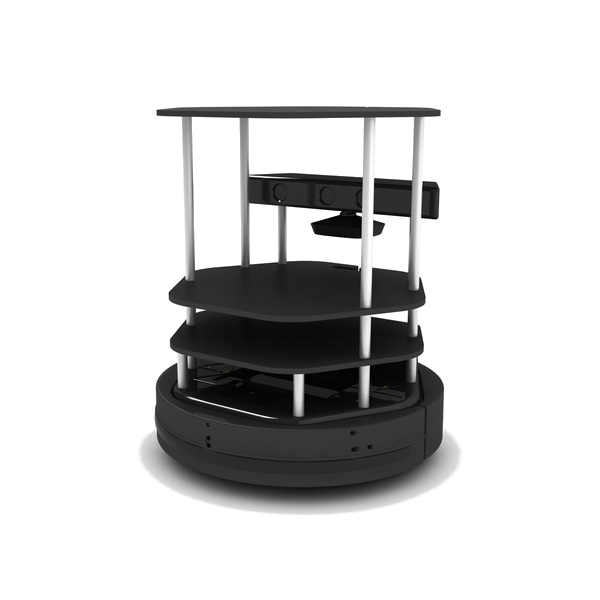
\includegraphics[scale=1.5]{./Figures/turtlebot.png}
	\caption{Vista frontal del Turtlebot 2 con un sensor Kinect acoplado\protect\footnotemark.}
	\label{fig:robotTurtlebot}
\end{figure}

\footnotetext{Imagen tomada de \url{https://static.generation-robots.com/6739-large_default/turtlebot-2-assembled-clearpathrobotics.jpg}}

\subsection{Clearpath Jackal}

El Jackal es un robot móvil 4x4 apto para uso en exteriores. Su robustez lo hace la elección preferida de muchas universidades a la hora de implementar soluciones de campo, principalmente debido a su resistencia total al polvo y al agua de lluvia.

\newpage

Posee una capacidad de carga de hasta 20 kg, lo que lo hace apto para cargar una importante cantidad de sensores, actuadores y manipuladores, tal como el ejemplo mostrado en la figura \ref{fig:robotJackal}.

\begin{figure}[ht]
	\centering
	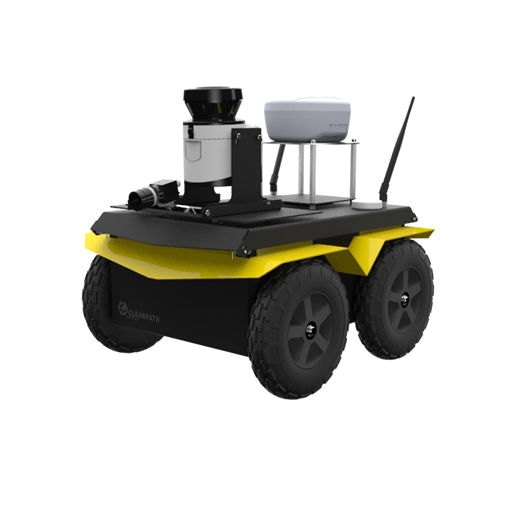
\includegraphics[scale=1.6]{./Figures/jackal.png}
	\caption{Vista frontal de la plataforma robótica Jackal con una batería de sensores instalados por el usuario\protect\footnotemark.}
	\label{fig:robotJackal}
\end{figure}

\footnotetext{Imagen tomada de \url{https://img.directindustry.es/images_di/photo-g/177123-10073681.jpg}}

\subsection{Fetch Freight 100 Base}

Fetch Robotics ofrece con el Freight 100 Base una plataforma robótica para uso en interiores \citep{PAPER:1}. Esta fue diseñada específicamente para moverse en edificios adaptados a personas en sillas de ruedas que cumplen con la normativa ADA o \textit{Americans with Disabilities Act} \citep{ACT:1}.

El Freight 100 incluye un sensor del tipo LIDaR 2D, que se puede apreciar en la figura \ref{fig:robotFreight}, lo que lo hace adecuado para tareas de navegación. Además, al estar basado en un robot industrial de carga, la plataforma Freight 100 está diseñada para soportar hasta 100 kg de peso, característica que no solo se impone por un amplio margen respecto a sus competidores del segmento, sino que le posibilita cargar con un manipulador industrial en su parte superior.

\begin{figure}[ht]
	\centering
	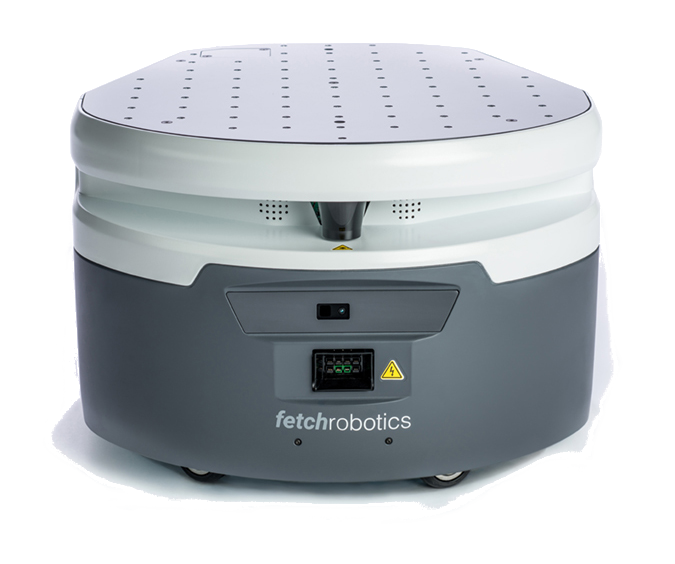
\includegraphics[scale=1.0]{./Figures/freight.png}
	\caption{Vista frontal de la plataforma robótica Fetch Freight donde se puede apreciar su sensor integrado del tipo LIDaR\protect\footnotemark.}
	\label{fig:robotFreight}
\end{figure}

\footnotetext{Imagen tomada de \url{https://www.dymesich.com/wp-content/uploads/2019/06/freight-100-low.jpg}}

\subsection{FESTO Robotino}

Robotino es un robot móvil comercializado por la compañía alemana FESTO Didactic. Está diseñado para entornos educativos, de entrenamiento y de investigación.
Esta plataforma dispone de un sistema de tracción omni que como su nombre sugiere, le otorga libertad de movimiento omnidireccional en dos dimensiones.

Asímismo, Robotino viene equipado de fábrica con una computadora tipo PC de grado industrial, lo que facilita su integración con elementos de hardware y software externos tales como cámaras, sensores y actuadores que utilicen el protocolo RS-232, RS-485 o USB. En la figura \ref{fig:robotRobotino} se puede apreciar al robot con una \textit{webcam} acoplada.

\begin{figure}[ht]
	\centering
	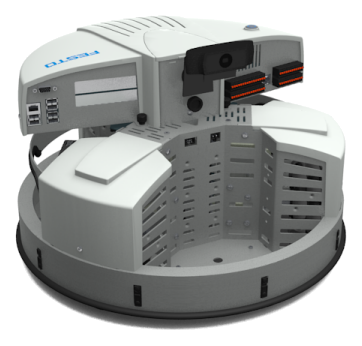
\includegraphics[scale=1.4]{./Figures/robotino.png}
	\caption{Vista frontal del Robot FESTO Robotino con un sensor externo acoplado\protect\footnotemark.}
	\label{fig:robotRobotino}
\end{figure}

\footnotetext{Imagen tomada de \url{https://www.festo-didactic.com/ov3/media/customers/1100/robotinohome.png}}


\subsection{Pioneer 3-DX}

El Pioneer 3-DX es un pequeño robot de tracción diferencial ideal para ser utilizado en entornos académicos ya sea en un laboratorio o en un salón de clases. Incorpora de fábrica cinco sensores del tipo SONAR al frente del robot como los que se pueden apreciar en la figura \ref{fig:robotPioneer}, encoders para las ruedas y un microcontrolador con firmware específico.

Su amplia superficie de carga permite transportar hasta 8 Kg, por lo que es un buen candidato para añadir sensores y actuadores extra, tales como cámaras o manipuladores de tamaño adecuado.

\begin{figure}[ht]
	\centering
	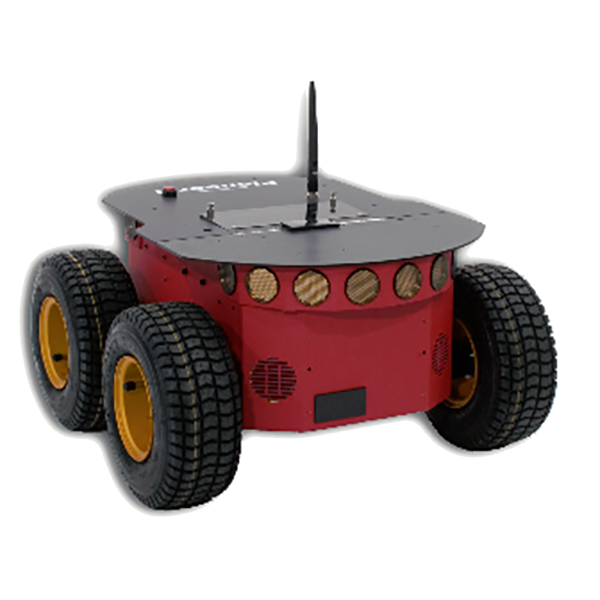
\includegraphics[scale=1.]{./Figures/pioneer.png}
	\caption{Vista frontal del Robot Pioneer donde se aprecian sus cinco sensores SONAR\protect\footnotemark.}
	\label{fig:robotPioneer}
\end{figure}

\footnotetext{Imagen tomada de \url{https://static.generation-robots.com/6645-large_default/robot-mobile-pioneer-3-at.jpg}}

\section{Motivación}

Los robots móviles expuestos en la sección anterior representan propuestas comerciales listas para usar que permiten a profesores, investigadores y alumnos concentrarse en el estudio o desarrollo de aplicaciones de la robótica móvil sin la necesidad de diseñar un robot desde cero para cada caso de uso específico. Gracias a esto, las instituciones o individuos que adquieren dichos equipos pueden ahorrar tiempo al concentrarse de inmediato en las tareas de interés para el estudio de la materia.

Es pertinente preguntar ¿por qué no todas las instituciones adquieren un robot comercial para el laboratorio de robótica?, la respuesta está en los costos asociados a la adquisición de estos equipos. Los robots destinados a investigación poseen precios prohibitivos para la mayoría de las instituciones educativas y por ende, son muy pocas las que se encuentran en condiciones de invertir en ellos.


\section{Objetivos}

En este trabajo se propone una plataforma de código abierto y con componentes disponibles en el mercado local paraguayo, destinada a la enseñanza de robótica móvil en instituciones educativas de nivel universitario.

\section{Alcance}

El alcance del presente trabajo involucra el desarrollo del firmware para el microcontrolador encargado de:
\begin{itemize}
	\item intermediar la comunicación entre la plataforma robótica ``Roomba 600'' y el framework de robótica ROS (\textit{Robot Operating System}).
	\item realizar la interfaz entre la unidad de medición inercial MPU6050 con ROS.
	\item implementar el \textit{port} de la biblioteca rosserial para ser utilizada con FreeRTOS y STM32Cube HAL en el lenguaje de programación C++.
\end{itemize}

Se incluye el desarrollo de software requerido para:
\begin{itemize}
	\item el paquete para ROS que brinda soporte básico para el robot propuesto "LuboBot", con sus sensores y actuadores.
	\item calcular la odometría del robot utilizando las lecturas de los encoders.
	\item la descripción del robot en formato URDF (\textit{Unified Robot Description Format}), requerido para representar correctamente el robot en la herramienta RViz.
	\item una imagen de Docker con todas las dependencias necesarias para utilizar el robot de manera encapsulada y sin la necesidad de modificar la configuración del sistema operativo del usuario.
	\item una sección extra en el repositorio oficial en GitHub con una Wiki con la documentación básica necesaria para iniciarse en el uso de la plataforma.
\end{itemize}

No se incluye con el presente trabajo:
\begin{itemize}
	\item ningún algoritmo de navegación local ni global.
	\item el código requerido para la conexión al microcontrolador mediante Ethernet.
	\item el diseño de una placa electrónica dedicada.
\end{itemize}